\documentclass[letterpaper,12pt,onecolumn]{article}
\usepackage[spanish]{babel}
\usepackage[latin1]{inputenc}
\usepackage{amsfonts}
\usepackage{amsthm}
\usepackage{amsmath}
\usepackage{mathrsfs}
\usepackage{empheq}
\usepackage{enumitem}
\usepackage[pdftex]{color,graphicx}
\usepackage{hyperref}
\usepackage{listings}
\usepackage{calligra}
\usepackage{algpseudocode} 
\DeclareMathAlphabet{\mathcalligra}{T1}{calligra}{m}{n}
\DeclareFontShape{T1}{calligra}{m}{n}{<->s*[2.2]callig15}{}
\newcommand{\scripty}[1]{\ensuremath{\mathcalligra{#1}}}
\lstloadlanguages{[5.2]Mathematica}
\setlength{\oddsidemargin}{0cm}
\setlength{\textwidth}{490pt}
\setlength{\textheight}{610pt}
\setlength{\topmargin}{-85pt}
\addtolength{\hoffset}{-0.3cm}
\addtolength{\textheight}{4cm}

\begin{document}
\thispagestyle{empty}
\begin{center}


\includegraphics[width=490pt]{figs/header.png}\\[0.5cm]

\textsc{\LARGE Parcial 3 - F\'isica I (FISI-1018) - Abril 26, 2016}\\[0.5cm]
\end{center}

Yo, \rule{10cm}{0.4pt}, con c\'odigo \rule{4cm}{0.4pt} de Uniandes,
acepto hacer este ex\'amen sin ayuda ni copia de fuentes no
permitidas (incluyendo libros, notas y cualquier dispositivo
electr\'onico),  sabiendo que hacer lo contrario va a ser considerado
como fraude (una falta grave que se sanciona hasta con suspenci\'on de la Universidad por
dos semestres como consta en el cap\'itulo X del reglamento general de
estudiantes). 

\begin{enumerate}


\item Un objeto de masa  $m$  est� unido mediante una cuerda a una
  rueda homog�nea de masa  $M$  y radio  $R$ (momento de inercia con
  respecto al centro de masa: $MR^2/2$). La cuerda no resbala
  sobre la rueda y �sta gira sobre su eje sin roce. Encuentre
\begin{itemize} 
\item  (10 puntos) La tensi�n de la cuerda
\item (15 puntos) La aceleraci�n de la masa.  
\end{itemize}

\item (25 puntos)
Un cilindro macizo de masa $M$ y radio $b$ (momento de inercia con
respecto al centro de masa: $Mb^2/2$) gira sin
  deslizamiento sobre un plano inclinado un \'angulo
  $\beta$. Encuentre la acelerac\'i\'on lineal con la que baja el
  cilindro. 

\item (25 puntos) Un hombre de masa $m$ va sobre sobre un carro que da vueltas
  sobre un riel circular de radio $R$ a velocidad $v$. Su centro de
  masa se encuentra a una altura $L$ del carro y sus pies est\'an
  separados una distancia $d$. El hombre est\'a mirando en la
  direcci\'on de movimiento. Calcule el peso que reposa sobre cada uno
  de sus pies.

\item 
(25 puntos)
Una esfera hueca de radio $r$ y masa $m$ (momento de inercia con
respecto al centro de masa: $mr^2$) se lanza desde una altura
$h$ por una pista como la mostrada en la Figura. Existe un poco de
fricci\'on de tal manera que la esfera baja rodando sin deslizamiento.
Despreciando las p\'erdidas de energ\'ia por la fricci\'on, encuentre
la altura m�nima de la cual se debe caer la esfera para que logre dar
la vuelta completa al bucle. 


\end{enumerate}

\begin{figure}[!h]
\begin{center}

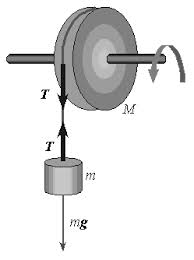
\includegraphics[scale=0.70]{torque.jpeg}
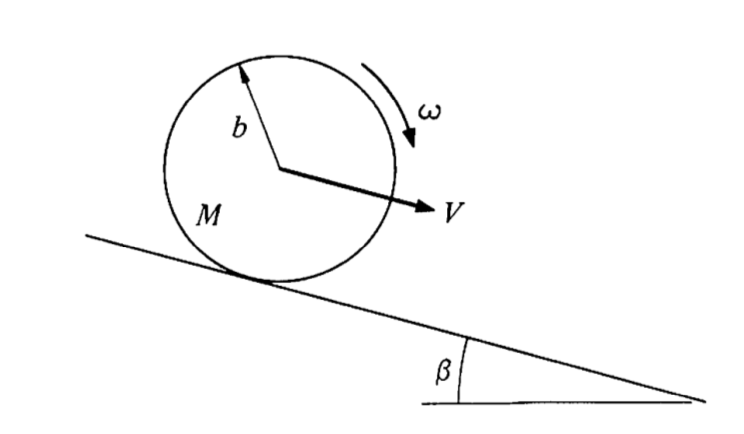
\includegraphics[scale=0.40]{cilindro.png}
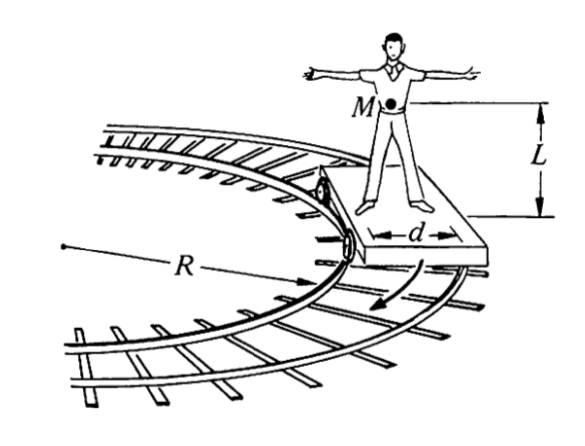
\includegraphics[scale=0.40]{riel.png}
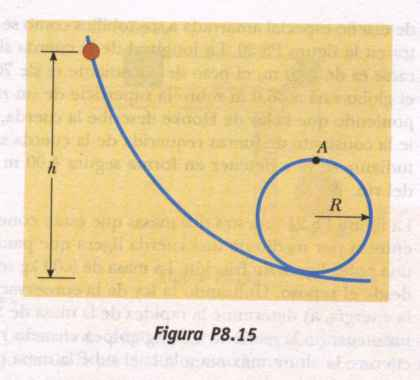
\includegraphics[scale=1.5]{montanarusa.jpg} 

\caption{Figuras para cada uno de los ejercicios.}
\end{center}
\end{figure}
{\small {\bf NOTA}: Todas las respuestas deben tener una justificaci\'on
f\'isica y matem\'atica adecuada. 100 puntos corresponden a una nota
de 5.0.}
\end{document}
